\documentclass{xetexCV}
%\usepackage[newsec,reorder]{cvsplitbib}
%\usepackage[newsec,reorder,export]{splitbib}
\usepackage[sorting=ydnt,maxnames=18,giveninits=true]{biblatex}
%\usepackage[bibstyle=publist]{biblatex}
\usepackage{xstring}
\usepackage{url}
\usepackage{fontspec}
\usepackage{booktabs}
%\usepackage{hyperref}

\usepackage{fancyhdr}
\pagestyle{fancy}
\lhead{Resume} 
\rhead{May 2019}
\chead{{\bf Dániel Varró}} 
\lfoot{} \rfoot{\bf \thepage} \cfoot{}

%\setmainfont[Ligatures={Common}, Numbers={OldStyle}]{Warnock Pro}
\setmainfont{Cambria}
\setsansfont{Calibri}
%\setsansfont{Frutiger LT Std}

%\plauthorname{Varr{ó}}

\addbibresource{bib/pcmember.bib}
\addbibresource{bib/varrodan.bib}

\renewcommand*{\mkbibnamegiven}[1]{%
\ifpartannotation{family}{self}{\textbf{#1}}{#1}}

\renewcommand*{\mkbibnamefamily}[1]{%
\ifpartannotation{family}{student}{#1\textsuperscript{*}}{%
\ifpartannotation{family}{self}{\textbf{#1}}{#1}}}

%\newcommand{\makeauthorbold}[1]{%
%  \DeclareNameFormat{author}{%
%    \ifthenelse{\value{listcount}=1}
%    {%
%      {\expandafter\ifstrequal\expandafter{\namepartfamily}{#1}{\mkbibbold{\namepartfamily\addcomma\addspace \namepartgiveni}}{\namepartfamily\addcomma\addspace \namepartgiveni}}
%      %
%    }{\ifnumless{\value{listcount}}{\value{liststop}}
%        {\expandafter\ifstrequal\expandafter{\namepartfamily}{#1}{\mkbibbold{\addcomma\addspace \namepartfamily\addcomma\addspace \namepartgiveni}}{\addcomma\addspace \namepartfamily\addcomma\addspace \namepartgiveni}}
%        {\expandafter\ifstrequal\expandafter{\namepartfamily}{#1}{\mkbibbold{\addcomma\addspace \namepartfamily\addcomma\addspace \namepartgiveni\addcomma\isdot}}{\addcomma\addspace \namepartfamily\addcomma\addspace \namepartgiveni\addcomma\isdot}}%
%      }
%    \ifthenelse{\value{listcount}<\value{liststop}}
%    {\addcomma\space}
%  }
%}
%
%\makeauthorbold{Varr{ó}}

 
%\renewcommand{\refname}{List of Publications}
%\setcounter{SBresetdepth}{2}
%\renewcommand{\refname}{}

%----------------------------- Service to Community ---------------------
%\begin{category}{Service to Scientific Community} 
%\begin{category}[CH]{Program Co-Chair}
%  \SBentries{sle2016-chair,icmt2014-chair,fase2013-chair,amt2012-chair,agtive2011-chair,grabats2010-chair,gtvmt2006-chair,grabats2006-chair}
%\end{category}
%
%\begin{category}[SC]{Steering Committee Member}
%  \SBentries{etaps2008-sc,etaps2013-sc}
%\end{category}
%
%\begin{category}[LO]{General Chair / Local Organizing Chair }
%  \SBentries{staf2013-chair,models2012-chair,sensus2009-lo,etaps2008-lo,models2007-chair,edcc2005-lo}
%\end{category}
%
%\begin{category}[JR]{Journals}
%  \SBentries{sosym,scp,ieee-tse,acm-tosem,sttt,ause}
%\end{category}
%
%\begin{category}[DS]{Opponent (External PhD reviewer)}
%  \SBentries{Ciccozzi,Kalauz,Hildebrandt,Zombori,Guta,Siikarla,Lundkvist,Meszaros,Gergely,Vidacs,Hettel,Sipos,Lukacsy,Hajdara}
%\end{category}
%
%\begin{category}[CH]{Chair of Doctoral Committee}
%  \SBentries{Vajk}
%\end{category}
%
%
%\end{category}
 
%----------------------------- PC Membership ---------------------

%\begin{category}{Program Committee Membership} 
%
%\begin{category}[SE]{Software Engineering}
%  \SBentries{icse2018-pc,fase2017-pc,%
%ase2016-pc,models2016-pc,ecmfa2016-pc,%
%ase2015-pc,models2015-pc,sle2015-pc,fase2015-pc,%
%ase2014-pc,models2014-pc,fase2014-pc,%
%  models2013-pc,ecmfa2013-pc,%
%  models2012-pc,ase2012-pc,ase2012tools-pc,icse2012tools-pc,%
%  fase2012-pc,csmr2012-pc,ecmfa2012-pc,icmt2012-pc,%
%  ase2011-pc,ase2011tools-pc%
%  models2011-pc,fase2011-pc,icmt2011-pc,ecmfa2011-pc,sofsem2011-pc,%
%  mbsdi2011-pc,melo2011-pc,%
%  models2010-pc,fase2010-pc,icmt2010-pc,ase2010-pc,modelsedu2010-pc,%
%  models2009-pc,fase2009-pc,icmt2009-pc,ase2009-pc,%
%  models2008-pc,icmt2008-pc,aramis2008-pc,%
%  wapl2007-pc,modelsedu2007-pc,modeva2007-pc,atem2007-pc,sac2007-pc,%
%  sac2006-pc,iwmec2006-pc,modeva2006-pc,atem2006-pc,gramot2006-pc,cmt2006-pc,gamma2006-pc,%
%  mtip2005-pc,gramot2005-pc%
%  }
%\end{category}
%
%\begin{category}[VT]{Visual Modeling Techniques and Tools}
%  \SBentries{gam2015-pc,vlhcc2014-pc,vlhcc2013-pc,vlhcc2012-pc,gtvmt2012-pc,%
%  vlhcc2011-pc,gtvmt2011-pc,%
%  gtvmt2010-pc,%
%  gtvmt2009-pc,%
%  gtvmt2008-pc,grabats2008-pc,%
%  gtvmt2007-pc,agtive2007-pc,%
%  fujaba2006-pc,fujaba2005-pc,grabats2004-pc%
%  }
%\end{category}
% 
%\begin{category}[DC]{Dependable Computing}
%  \SBentries{ewdc2011-pc,dsn2009-pc,edcc2006-pc,icdcs2006-pc}
%\end{category}
%
%\begin{category}[FM]{Formal Methods}
%  \SBentries{icgt2014,icgt2012-pc,icgt2012ds-pc,%
%  ictac2011-pc,icgt2010-pc,ictac2010-pc,%
%  fm2009-pc,%
%  icgt2008-pc,pngt2008-pc,%
%  icgt2006-pc,gtvc2006-pc,gtvc2005-pc}
%\end{category}
%
%\begin{category}[ED]{Education}
%	\SBentries{models2010edu-pc,models2007edu-pc}
%\end{category}
%\end{category}

%\nocite{*}
%\SBtitlestyle{bar}
%\SBsubtitlestyle{none}

%\begin{category}{Publications} 
%\begin{category}[B]{Books and Book Chapter (Total: 8)}
%  \SBentries{fmi2004,nagl65-2010,bpel2sal-sensoria-book,sensoria-uml,SENSORIABook:AdvancesInGT,mdegt2005_ggzvvv,caise2011-revised,fmic2005_pv}
%\end{category}
% 
%\begin{category}[J]{Refereed Journals (Total: 21)}
%%  \SBentries{ist2015,scp2015,ause2014,sosym2014-trace,sosym2012-tools,sosym2011-cdt,sosym2011-csp,Bergmann-sttt10,Gilmore-sosym10,Rath-sosym09,sosym2008-mtbe,ijcsse08-kgv,scp-2007,sosym2005_bhtv,hiradas2006-hvv,sosym2005_db,sosym2004_mc,FundInf2003_ghv,pp2003_as,sosym2003_vpm,SCP2002} 
%  \SBentries{SCP2002,sosym2003_vpm,pp2003_as,FundInf2003_ghv,sosym2004_mc,sosym2005_db,hiradas2006-hvv,sosym2005_bhtv,scp-2007,ijcsse08-kgv,sosym2008-mtbe,Rath-sosym09,Bergmann-sttt10,Gilmore-sosym10,sosym2012-tools,sosym2011-cdt,sosym2011-csp,scp2015,ause2014,ist2015,sosym2014-trace} 
%\end{category}
%
%\begin{category}[C]{Peer Reviewed Conference Papers (Total: 48)}
%%  \SBentries{ase2014,models2014-iqd,models2014-stream,sle2014,csmr2014,models2013,models2012,ecmfa2012,icgt2012-ts,icst2012,tools2012,ase2011-dse,ase2011-mtslice,ase2011-tool,vlhcc2011,ecmfa2011,icmt2011,models-2010-incquery,ServiceWave2011,SEFM10:back-ann,Bergmann-icmt08,Horvath-models09,Rath-models09,icgt08-bhrv,Gonczy-mdwe08,icmt08-rbov08,Rath-vlhcc08,agtive07-vhv,isas-2007-kv,sac2007-vb,sac06_vtcl,sac06_plugin,isas2006_kvn,models2006-varro,icgt2006,isas05_bvp,fase2005_eeltvv,vlhcc05_vsv,wicse2004_bhtv,GI2004,icgt2004_rsv,uml2004_meta,esec03_bhtv,uml2003_tool,ASE2002,ICGT2002-GHV02,ICGT2002-SC,UML2002} 
%  \SBentries{UML2002,ASE2002,ICGT2002-GHV02,ICGT2002-SC,%
%esec03_bhtv,uml2003_tool,%
%wicse2004_bhtv,GI2004,icgt2004_rsv,uml2004_meta,%
%isas05_bvp,fase2005_eeltvv,vlhcc05_vsv,%
%sac06_vtcl,sac06_plugin,isas2006_kvn,models2006-varro,icgt2006,%
%agtive07-vhv,isas-2007-kv,sac2007-vb,%
%icgt08-bhrv,Gonczy-mdwe08,icmt08-rbov08,Rath-vlhcc08,%
%Bergmann-icmt09,Horvath-models09,Rath-models09,%
%SEFM10:back-ann,models-2010-incquery,%
%ase2011-dse,ase2011-mtslice,ase2011-tool,vlhcc2011,ecmfa2011,icmt2011,ServiceWave2011,%
%models2012,ecmfa2012,icgt2012-ts,icst2012,tools2012,models2013,%
%ase2014,models2014-iqd,models2014-stream,sle2014,csmr2014} 
%\end{category}
%
%\begin{category}[O]{Other Conference Papers (Total: 3)}
%  \SBentries{dasc2010-hvs,Daboczi-AWSN2013,dasc2014}
%\end{category}
%   
%\begin{category}[W]{Refereed Workshop Papers (Total: 42)}
%%  \SBentries{cmseba2014,mpm2014,oss4mde2014,bigmde2014,bigmde2013,ocl2012,amt2012-query,eceasst2010-guided,eceasst2011-type,SEFM10ToolDemo:back-ann,Bergmann-gtvmt09,Gonczy-safecomp08,gramot08-borvv,gtvc2006-gkv,GT-VMT2007-hvv,efts-2007-kgv,cmt2006,gtvmt06_dpv,wsmate2006,gramot2005_tax,dspd2006_rv,pngt2006-vv,models2006-edu,gramot2005_adapt,gramot2006-vvs,mtip2005,gtvmt04_gsv,grabats2004_vfv,gtvmt04_vv,cbse03_bhtv,DDECS2003_tvp,csduml2003,GRABATS2002,edcc2002_svp,GTVMT2002,FMOODS2002,AGT2002,WTUML01,GRATRA2000,DDECS2000}
%  \SBentries{GRATRA2000,DDECS2000,WTUML01,%
%edcc2002_svp,GTVMT2002,FMOODS2002,AGT2002,GRABATS2002,%
%cbse03_bhtv,DDECS2003_tvp,csduml2003,%
%gtvmt04_gsv,grabats2004_vfv,gtvmt04_vv,%
%gramot2005_adapt,gramot2006-vvs,mtip2005,%
%cmt2006,gtvmt06_dpv,wsmate2006,gramot2005_tax,dspd2006_rv,pngt2006-vv,models2006-edu,gtvc2006-gkv,%
%GT-VMT2007-hvv,efts-2007-kgv,%
%Gonczy-safecomp08,gramot08-borvv,%
%Bergmann-gtvmt09,%
%SEFM10ToolDemo:back-ann,eceasst2010-guided,%
%eceasst2011-type,%
%ocl2012,amt2012-query,%
%Kolovos-bigmde2013,Izso-bigmde2013,%
%bigmde2014,cmseba2014,mpm2014,oss4mde2014,vao2014}
%\end{category}
%
%\begin{category}[I]{Invited Papers (Total: 5)}
%%  \SBentries{csmr2012-invited,models09-edu,agtive07-toolcontest,Wirsing-isola08,easst2006-etv}
%  \SBentries{easst2006-etv,Wirsing-isola08,agtive07-toolcontest,models09-edu,csmr2012-invited}
%\end{category}
%
%\begin{category}[E]{Edited Volumes (Total: 7)}
%%  \SBentries{icmt2014,fase2013,amt2012,agtive2011,grabats2010,icgt2006-grabats,gtvmt2006}
%  \SBentries{gtvmt2006,icgt2006-grabats,grabats2010,agtive2011,amt2012,fase2013,icmt2014}
%\end{category}
%
%\end{category}


  
\cvname{D\'aniel Varr\'o}
%\cvimage{figures/varro.jpg}
\cvimage{figures/VarroD-2015-small.jpg}
%\institution{Contact Address:} 
%\contactaddress{Arany J\'anos u. 77. fszt.1 Budapest, 1221, Hungary (until 20/08/19) \\
%80 Chesterfield Avenue, Westmount QC, Canada, H3Y 2M7 (from 20/08/19) \\ 
%\emph{Please send all relevant communications also in email because of my changing address}} 
%\phonenumber{+36-30-2438706}
%\phonenumber{+1-514-5831084}
%\email{daniel.varro@gmail.com}

\institution{Contact Address:} 
\contactaddress{3480 Rue University, McConnell Engineering Building \\
Department of Electrical and Computer Engineering \\
McGill University \\
Montreal, QC, Canada, H3A 0E9}
\phonenumber{+1-514-3983681}
\email{daniel.varro@mcgill.ca}

%\institution{Contact Address: }
%\contactaddress{Electrical and Computer Engineering Department\\
%McGill University \\
%3480 University Street \\
%Montreal, QC, H3A0E9\\
%Canada}
%\email{daniel.varro@mcgill.ca}

%\contactaddress{Department of Measurement and Information Systems \\
% Budapest University of Technology and Economics \\
%Magyar tud\'osok krt. 2 \\
%Budapest, H-1117 \\
%Hungary}
%\email{varro@mit.bme.hu}
%\website{http://www.inf.mit.bme.hu/en/members/varro}  
%\url{http://www.mit.bme.hu/~varro}

\hyphenpenalty=10000

% Set the Font to Warnock Pro and Frutiger LT Std
%\setmainfont[Ligatures={Common}, Numbers={OldStyle}]{Fontin}
%\setsansfont{Fontin Sans}

\begin{document}
\makecvtitle

\thispagestyle{empty}

\cvsection{Education and Degrees}
Doctor of Science (DSc); \years{2013}Hungarian Academy of Sciences  
%\newline This degree is a formal prerequisite of full professorship in Hungary. \\


Habilitation; \years{2011}Budapest University of Technology and Economics (in short: BME) 

PhD \years{2004}in Software Engineering (official name: Technical Informatics);
BME %Budapest University of Technology and Economics \\

MSc \years{2000}in Software Engineering (official name: Technical Informatics); 
BME %Budapest University of Technology and Economics  

\cvsection{Academic Positions}
Professor \years{2016 - }, Electrical and Computer Engineering (ECE) Department, McGill University

Research Chair \years{2015 - 2020} of MTA-BME Lendulet Cyber-Physical Systems Research Group \\ Hungarian Academy of Sciences 

Professor, \years{2014 - } Dept. of Measurement and Inf. Systems, BME  (on leave)

Visiting Professor, \years{2014} Dept. of Computer Science, McGill University, Canada

%Visiting Professor \years{2014}, D\'epartemente d'informatique et de recherche op\'ertionnelle, Universit\'e de Montr\'eal, Canada
Visiting Professor, \years{2014} DIRO, Universit\'e de Montr\'eal, Canada

Associate Professor (tenured), \years{2009 - 2014} Dept. of Measurement and
Inf. Systems, BME 	

Assistant Professor\years{2005 - 2009}, Dept. of Measurement and
Information Systems, BME 

Lecturer\years{2003 - 2005}, Dept. of Measurement and Information
Systems, BME

\cvsection{Industrial Positions and Entrepreneurship} 
Co-founder of IncQuery Labs Ltd. (Co-founder and Strategic advisor) \years{2013-}  \\
Co-founder of OptXware Ltd. (Vice-President of Research and Development) \years{2006-2014} \\

\cvsection{Research Interests}
Model based software and systems engineering, Cyber-physical systems, \\
Formal methods, Critical embedded systems, Graph-based tools and databases
%A draft research statement is available at:
%\url{https://dl.dropboxusercontent.com/u/62723032/LERO/VarroD_ResearchStatement.pdf}
%Application areas: critical embedded systems, service-oriented applications


\cvsection{Research Visits} 
Universit\'e de Montr\'eal \years{2014} (Prof. Houari Sahraoui) and McGill University (Prof. Hans Vangheluwe),  6 months


TU Berlin, Germany (2x 1 month, with Prof. Hartmut Ehrig, SEGRAVIS Grant)
\years{2004, 2005} 

Univ. Paderborn, Germany \years{2003} (3 months, with Prof. Gregor Engels,
SEGRAVIS) \

SRI International, US (4 months, with Dr. John Rushby) \years{2001} 

\cvsection{Awards and Honors} 
%\emph{The 5 award winning papers (or their journal extensions) are included in my application package}

\textbf{Distinguished Reviewer Award} \years{2018} (at ICSE 2018: 40th (IEEE/ACM) International Conference on Software Engineering)

\textbf{Best Tool Paper Award} \years{2018} at MODELS 2018 (ACM/IEEE 21st Int. Conference on Model Driven Engineering Languages and Systems (1 out of 10 tool papers)

\textbf{EASST Best Paper Award} \years{2018} (at ETAPS 2018: European Joint Conferences on Theory and Practice of Software: selected 1 out of over 140 papers)

\textbf{Csanád Imreh Award} \years{2017} (by OTDT Hungary): I was the first ever awardee of the prize (awarded in the field of software engineering and computer science for Hungarian researchers below the age of 41) commemorating the Hungarian computer scientist who tragically died in 2017 at the age of 41.  

ACM \years{2016} \textbf{Distinguished Paper Award} (at MODELS 2016: 19th IEEE/ACM International Conference on Model Driven Engineering Languages and Systems) 

IEEE \years{2016} \textbf{10-Year Most Influential Paper Award} \newline (at VL/HCC 2016: IEEE Symposium on Visual Languages \& Human-Centric Computing for a paper presented at VL/HCC 2005 conference) 

Springer \years{2014} \textbf{10-Year Most Influential Paper Award} \newline (at MODELS 2014: 17th IEEE/ACM International Conference on Model Driven Engineering Languages and Systems for a paper presented at UML2004 conference) 

\textbf{Best Paper Award} \years{2014} (at IEEE CSMR-WCRE 2014 Software Evolution Week) 

\textbf{STEM Award} \years{2014} by Tempus Foundation for innovative education methods (introducing Apache VCL cloud based labs)

Springer \years{2013} \textbf{Best Paper Award} (MODELS 2013: 16th IEEE/ACM International Conference on Model Driven 
Engineering Languages and Systems) 

ACM \years{2011}\textbf{Distinguished Paper Award} (ASE 2011: 26th IEEE/ACM International Conference on Automated Software Engineering) 

\textbf{J\'anos Bolyai Scholarship} \years{2010-2013}(Design and Analysis Techniques for the Certification of Model Transformations): A national award of the Hungarian Academy of Sciences for young scholars. It can be awarded
at most twice.

\textbf{Distinguished Tutor}: \years{2009} Bi-annual award for the supervisionof MSc students carrying out early research with 3 awardees in Computer Science biannually. It requires 10 years of successful tutoring (I became the youngest ever awardee). 

Springer \years{2009}\textbf{Best Paper Award} and ACM \textbf{Distinguished Paper Award} \newline (MODELS
2009: The 12th IEEE/ACM International Conference on Model Driven Engineering Languages and
Systems) 

\textbf{J\'anos Bolyai Scholarship} \years{2005-2008} (Design and Analysis Techniques
for Automated Model Transformations) 

\textbf{J\'anos Kem\'eny Prize } \years{2003}(An annual
award in Hungary for young scholars issued by John von Neumann Computer Society)


\cvsection{Invited talks (34)}
\emph{Keynote talk}: Automated \years{2017} Graph Model Generation for Smart and Safe Cyber-Physical Systems (Consortium for Software Engineering Research CSER 2017) \\

\emph{Keynote Talk}: \years{2016} Incremental Queries and Transformations: From Concepts to Industrial Applications  (SOFSEM 2016 conference) 

Graph-based  Design and Analysis Tools for Smart and Safe Cyber-Physical Systems (NASA Jet Propulsion Lab) 

Incremental Queries and Reactive Transformations (DSM-TP 2017 Summer School, Montreal, Canada)

Formal Verification and Validation in Domain-Specific Languages (DSM-TP 2017 Summer School, Montreal, Canada)
	
Model-based Tools for Engineering Cyber-Physical Systems (McGill University Professor Talks)

Scalable  Graph-based techniques for smart cyber-physical systems (Papyrus Industrial Consortium)

Models and Queries for Smart and Safe Cyber-Physical Systems (CSCS 2016 Conference, Szeged)

Challenges for Smart and Trustworthy Cyber-Physical Systems (Ericsson University Day 2016 Budapest)

Incremental Model Queries and Transformations (DSM-TP International Summer School; DSM-TP 2016) \\

EMF/Ecore-based DSL engineering \years{2015} (at Dagstuhl \#15062:  Domain-Specific Languages)

EMF-IncQuery: Incremental Evaluation of Model Queries (DSM-TP 2015)  

VIATRA: Advanced Tools by Reactive Transformations (DSM-TP 2015) \\

\emph{Plenary Talk}: Generic and Meta-Transformations \years{2014} (Most Influential Paper Presentation at @MODELS 2014, Valencia, Spain)

Incremental Model Queries over the Cloud (SERENE 2014 Autumn School, Hungary)


EMF-IncQuery: Incremental Evaluation of Model Queries (DSM-TP 2014)


Traceability Challenges in Design Tools for Avionics (DSM-TP 2014) 

Distributed Incremental  Model Queries over the Cloud: Engineering and Deployment Challenges 
(Keynote at CloudMDE 2014 Workshop @MODELS 2014)


Distributed Incremental Model Queries (GT-VMT 2014 Workshop @ETAPS 2014) \\


Validation of Complex Domain-Specific Modeling Languages \years{2013} (at Dagstuhl Seminar 13211 
Automatic Reasoning on Conceptual Schemas)


V\&V Challenges for Models, Queries and Transformations in Design Tools for Avionics (VOLT 2013 Workshop)


Model queries for secure collaborative modeling (EternalS 2013 Workshop) \\

\emph{Keynote speaker} \years{2012} at 16th European Conference on Software Maintenance
and Reengineering (CSMR 2012, Szeged, Hungary) 

Developing Design Tools for Critical Embedded Systems: A Model Transformation Playground
(at RISC, Hagenberg, Austria) \\

Designing Domain-Specific Languages (at University of Szeged, Hungary)
\years{2010} \\

Model driven \years{2009} development of configuration tables (at Rockwell Collins, US)

Model transformation development (at SENSUS Summer School, HU)

Service deployment by model transformation (at SENSUS Summer School, HU)
\\

Precise model transformations for tool integration (at TU Berlin, Germany)
\years{2008} \\

Model transformation by example (at ISIS, Vanderbilt University, US)
\years{2007} 

Model-Driven Deployment of Services to Standards Compliant Reliable
Middleware (at Dagstuhl Seminar 07061 Autonomous and Adaptive Web Services)
\\

The VIATRA2 model transformation framework (at TU Darmstadt, Germany)
\years{2004-2003} 

Towards Automated Formal Verification of Visual Modeling Languages
%by Model Checking 
(at Dagstuhl Seminar 04101 Language Engineering for Model-Driven Software Development) 

Model checking visual modeling languages (at SRI International, US) %\years{2003} \\

\cvsection{Membership in Professional Societies and Committees}
\textbf{Member}: \years{2018-}  The McGill Sustainability Systems Initiative (MSSI)\\
\textbf{Member}: \years{2016-}  McGill Institute for Aerospace Engineering (MIAE)\\
\textbf{3x Elected member}: \years{2011-} Informatics Committee of Hungarian Academy of Sciences \\
\textbf{Vice president}: \years{2009-2015} John von Neumann Computer Society \\
\textbf{Member}: IEEE Computer Society \years{2006-}

\newpage

\cvsection{Projects and Grants} 
\lhead{Third party funding} 


\cvsubsection{Canadian Projects (as PI or co-PI)}
\textbf{NSERC-CRD}: \years{2018 - 2023} Digital Multidisciplinary Analysis and Design Optimization Platform for Aeroderivative Gas Turbines, NSERC Collaborative Research and Development Grant, PI: M. Kokkolaras (McGill), co-PIs: H. Moustapha (ETS), 
D. Varr\'o:  Total/own funding: 1,177,500 CAD / 294,375 CAD (25\%)\\
\textbf{NSERC-SDG}: \years{2017} LiveIDE: Live Integrated Development Environment for Software-Intensive Communication Systems, PI: D. Varr\'o, co-PIs: G. Mussbacher, J. Kienzle (McGill), H. Sahraoui, E. Syriani (UdeM): Submitted as a Strategic Partnership Grant, recommended for funding by NSERC as a Collaborative Research and Development Grant with Ericsson. The CRD contract was not signed as the Ericsson project lead left the company: Total funding: 571,275 CAD\\
\textbf{NSERC-DG}: \years{2016 - 2021} Model-based Design and Validation Techniques for
Smart and Safe Cyber-Physical Systems (RGPIN-2016-04573), NSERC Discovery Grant, PI, own funding: 230,000 CAD \\
\textbf{McGill Startup Fund}: \years{2016 - 2019} Initial research support: 55,000 CAD \\
\textbf{McGill}: \years{2016 - 2019} 4 teaching support funds by EUSF: total around 7,500 CAD \\

\cvsubsection{Collaborative European Projects (as Site Leader or Research Coordinator at BME)}
\textbf{MONDO}: \years{2013 - 2016} Scalable Modelling and Model Management 
on the Cloud (EU-FP7-ICT-STREP, own funding: 420,000 EUR)  \\
\textbf{E-Freight}: \years{2010 - 2013}European e-Freight Capabilities for
Co-modal Transport (EU-FP7-SST-IP, own funding: 260,000 EUR)  \\
\textbf{SecureChange}: \years{2009 - 2012}Security Engineering for Lifelong
Evolvable Systems (EU-FP7-FET-IP, 231101-2009, own funding: 250,000 EUR)  \\ 
\textbf{DIANA}: \years{2006 - 2010}Distributed, equipment Independent
environment for Advanced avioNic Applications (EU-STREP, FP6-2005-Aero-1, own funding: 410,000 EUR) \\
\textbf{SENSORIA}: \years{2005 - 2010}Software Engineering for Service Oriented
Overlay Computers (FP6 European IP, IST-016004, own funding: 300,000 EUR)  

\cvsubsection{Hungarian National Projects (as PI)}


\textbf{MTA-BME Lend\"ulet} \years{2015-2020} Cyber-Physical Systems Research Group, 520 000 EUR\\

\textbf{CERTIMOT}: \years{2010-2014}Design and Analysis Techniques for
Certifiable Model Transformations (ERC-HU-09: Starting Grant, 370 000 EUR: My
ERC Starting Grant proposal went to the final round at EC with a score of 7/8;
%and it was recommended for funding but became out of budget, 
finally it was partially funded by the Hungarian Research Agency.


\cvsubsection{Industrial Research Grants and Projects} 

\textbf{TRANS-IMA}: collaborative project with \years{2012-2014}\textbf{Embraer} on
model-driven avionic design tools (funding: 200 000 EUR) \\

Collaborative project with \years{2013-2014}\textbf{Ericsson} on
modeling and verification of statecharts (funding: 20 000 USD)\\

\textbf{IBM Faculty Award}: \years{2007}A framework for the model-driven design
and analysis of standards-compliant IT infrastructure management (by IBM TJ Watson Research Centre,
funding: 20,000 USD)  \\

\textbf{IBM Faculty Award}: \years{2006}Model based deployment of services to
standards-compliant reliable IBM middleware (by IBM TJ Watson,
funding: 10,000 USD)  \\

\textbf{IBM Faculty Award}: \years{2005}Model Transformation Engineering as a
complement to IBM Process Modeling Technologies (by IBM TJ Watson, 
funding: 6,000 USD)  \\

Two collaborative projects with \years{2006-2010}\textbf{Nokia Research Centre}
on high-availability service platforms, and on MDD%model-driven development
techniques (funding: 40 000 EUR)\\

%\textbf{Total own funding}: approx. 2.2 million EUR \\
\textbf{Total acquired own funding}: approx. 3.1 million EUR \\
%\textbf{Total acquired own funding}: approx. 4.65 million CAD\\
(This excludes funding I secured as a co-founder of IncQuery Labs Ltd, which also exceeds 800K EUR, but not reported in the current CV.)
%(This excludes funding I secured as a co-founder of IncQuery Labs Ltd, which exceeds 1.2 million CAD, but not report due to non-disclosure agreements.)

\cvsection{Further Project Participation} 

\cvsubsection{Collaborative Research Projects (as Contributor)}
%\textbf{NECSIS}: \years{2014} (An Automotive Partnership Canada project)  \\
\textbf{INDEXYS}: \years{2009-2011}INDustrial EXploitation of the genesYS
cross-domain architecture (ARTEMIS-2008-1-100021)  \\
\textbf{RESIST}: \years{2006-2008}Resilience for Survivability in IST (EU-FP6
Network of Excellence)  \\
\textbf{DECOS}: \years{2004-2007}Dependable Embedded Components and Systems (FP6
European IP) \\
\textbf{SEGRAVIS}: \years{2002-2006}Syntactic and Semantic Integration of
Visual Modelling Techniques (Research Training Network) 

\cvsubsection{National Research Projects (as  Contributor)}

EC-Conforming \years{2005-2006} Certification of Safety Equipments for Hungarian
Railways (GVOP-2004-3.1.1) \\
Operation Research Methods \years{2001-2003} for the Analysis and Verification
of IT Systems (OTKA T038027) \\ 
Framework \years{2000-2002} for the Development and Testing of Dependable,
Safety-Critical Systems (IKTA-00065/2000) \\  
Formal Methods in Informatics (MEH 96/2000) \years{2000-2001} \\
Automated Verification \years{1999-2001} and Validation of UML Models for IT
Systems (OTKA T030804) 

\cvsubsection{National Projects on innovative exploitation of academic results (as Major Contributor)}

An MDA \years{2005-2007}based product family for service dependability and
optimization (GVOP-2005-3.3.1, in Hungarian)  



\cvsection{Major Open Source Software Projects}

VIATRA \years{2004-} Model Transformation Framework (Founder): Official open source project hosted by the Eclipse Foundation \newline
\url{http://www.eclipse.org/viatra} 

EMF-IncQuery: \years{2010-2016} Incremental queries over EMF models (Co-founder) 
%\url{http://www.eclipse.org/incquery/} \\

MASSIF: \years{2014-} Matlab Simulink Integration Framework for Eclipse (Co-founder) \newline 
\url{https://github.com/viatra/massif} 

%Eclipse Committer \years{2005-}(now in Modeling project) 
%\\

%Key contributor to several other research prototypes 
%CheckVML: \years{2002-2004}Model checking for graph transformation systems
%\\

\newpage

\cvsection{Significant University Duties}
\lhead{Teaching and University Duties} 

\cvsubsection{Departmental Committees (at McGill)}
\textbf{Program director}, Software engineering co-op program \years{2018-}\\
\textbf{Member}, Undergraduate Advising Committee, \years{2018-} \\
\textbf{Member}, Curriculum Committee \years{2018-}\\
\textbf{Member of Qualifying Exam Committee}: \years{2018} M\'arton B\'ur\\
\textbf{Member}, Faculty Search Curriculum \years{2017-19}\\
\textbf{Member}, Promotions and Reappointment Committee \years{2017-18}\\
\textbf{Member of Qualifying Exam Committee}: \years{2017} Anastasios Alexandridis \\
\textbf{Member}, Chairman's Advisory Commitee \years{2016-18}\\
\textbf{Member}, Departmental Tenure Commitee \years{2016-18}\\
\textbf{Member}, Graduate Student Financing Committee \years{2016-17}\\

\cvsubsection{University Committees (at McGill)}
\textbf{Representative of Engineering Faculty}, \years{2017-} Council of Graduate and Postdoctoral Studies (CGPS) \\
\textbf{Member}, Committee on Student Exchange and Study Abroad \years{2018-} \\
\textbf{Pro-Dean}, \years{2018} Art History \& Communication Studies, McGill University \\
\textbf{Member}, GitHub Enterprise evaluation committee \years{2017-}\\

\cvsubsection{Major Academic Duties in Hungary}
\textbf{External member}: \years{2014-16} Informatics Doctoral School, University of Szeged  \\
\textbf{Core member}: \years{2014-} Informatics Doctoral School, BME   \\
\textbf{Specialization coordinator}: \years{2014-2016} Systems Engineering Specialization (UG), BME   \\
\textbf{Operative lead}: \years{2012-2016} Fault Tolerant Systems Research Group, BME   \\
\textbf{Member}: \years{2012-2016} Operative Committee, Dept. of Measurement and Inf. Systems, BME   \\

\cvsection{Graduate Supervision and Tutoring}
%\cvsubsection{PhD students (main supervisor)}

\textbf{PhD students (main supervisor)}: 11 supervised (5 defended), see \autoref{tab:phd-supervised} \\
\textbf{PhD students (co-supervisor)}: 8 students (4 defended), see \autoref{tab:phd-cosupervised} \\
\textbf{MEng/MSc thesis students}: 28 (co-)supervised (23 defended), see \autoref{tab:msc-supervised} \\
%\textbf{Undergraduat students (at McGill)}: 35 students, 9 Design projects (ECSE 456/457), 6 SURE (Summer Undergraduate Research in Engineering) projects, see \autoref{tab:ug-supervised} \\

\textbf{International Awards Won by PhD students}: 4 major international prizes \\
\emph{G. Sz\'arnyas}: ACM Student Research Competition (SRC): 2nd place at SIGMOD 2018 (main scientific forum in database research), \\
\emph{C. Debreceni}: ACM SRC: 1st Prize at MODELS 2017;\\
\emph{G. Sz\'arnyas}: ACM SRC: 1st Prize at MODELS 2016; \\
\emph{G. Sz\'arnyas}: Best Presentation Award at STAF 2014 Doctoral Symposium \\


\textbf{Selected workplaces of past graduate students}: Google (3 students), Morgan Stanley, Ericsson, ThyssenKruppPresta, PwC, Nokia-Siemens Networks, 
%European Chemical Agency, Trendency, 
IncQuery Labs, Lufthansa Systems, Siemens, National Instruments \\

\textbf{Tutoring MSc students on a national-level scientific competition}: \\
23 scientific reports; 3x 1st prize (on national level), 3x 3rd prize (on national
level), 12x 1st prize (on faculty level), %8x second prize (on faculty level)) 
\textbf{Distinguished Tutor}  \\%(youngest awardee; requires 10 years of successful tutoring) \\
%Distinguished Tutor (2009) (youngest ever awardee; requires 10 years of highly successful tutoring) \\

\textbf{Comments:} A boldface single year denotes the year of completed PhD defense, a period denotes years of supervision \\

% Please add the following required packages to your document preamble:
% \usepackage{booktabs}
\begin{table}[htb]
\begin{tabular}{@{}lllp{6cm}p{4cm}@{}}
\toprule
\textbf{Name} & \textbf{Inst.} & \textbf{Year} & \textbf{Research Topic} & \textbf{Current job} \\ \midrule
M\'arton B\'ur   & McGill  & 2016-   & Distributed Graph Queries for Runtime Monitorong of Cyber-Physical Systems & PhD student \\
Csaba Debreceni & BME  & 2014-19 &  Advanced Techniques and Tools
for Secure Collaborative Modeling & PhD candidate \newline (defense in July 2019)\\
Oszk\'ar Semer\'ath & BME  & 2014-19 &  Formal Validation and Model Generation
for Domain-Specific Languages & PhD candidate \newline (defense in June 2019)\\
G\'abor Sz\'arnyas & BME  & 2014-19 &  Query, Analysis, and Benchmarking Techniques
for Evolving Property Graphs of Software Systems & PhD candidate \newline (defense in June 2019)\\
Zolt\'an Ujhelyi & BME  & \textbf{2017} &  Program Analysis Techniques for Model Queries and Transformations & Senior MDE Expert at IncQuery Labs\\
Andr\'as Sz. Nagy & BME  & 2015-17 & Design Space Exploration & Associate at MSCI Inc.\\
Benedek Izs\'o & BME  & 2012-14 &  Benchmarking of Graph Queries & Software Developer at IP Systems\\
\'Akos Heged\"us & BME  & \textbf{2014} &  Back-annotation of Execution Sequences by Advanced Search and Traceability Techniques & CTO at IncQuery Labs\\
G\'abor Bergmann & BME  & \textbf{2013}   &  Incremental Model Queries
in Model-Driven Design & Assistant professor at BME, J. Bolyai Scholar \\
\'Akos Horv\'ath & BME  & \textbf{2013} &  Model-Driven Development Techniques for
Integrated Modular Avionics Systems & CEO at IncQuery Labs \\
Istv\'an R\'ath   & BME  &  \textbf{2011} & Event-driven Model Transformations in
Domain-specific Modeling Languages & CEO at IncQuery Labs \\ \bottomrule
\end{tabular}
\caption{PhD students (as main supervisor)}
\label{tab:phd-supervised}
\end{table}


\begin{table}[htb]
\begin{tabular}{@{}lllp{3cm}p{7cm}@{}}
\toprule
\textbf{Name} & \textbf{Inst.} & \textbf{Year} & \textbf{Main supervisor} & \textbf{Current job} \\ \midrule
L\'aszl\'o G\"onczy & BME & \textbf{2019}  & Tam\'as Bartha & lecturer at BME, CEO of Quanopt Ltd.\\
Krist\'of Marussy & BME & \textbf{2018-}  & Istv\'an Majzik & PhD student at BME, Graduate research trainee at McGill \\
Th\'eo Le Calvar & ESEO & \textbf{2018}  & Fr\'ed\'eric Jouault & PhD student at ESEO Angers, Graduate research trainee at McGill \\
\'Akos Hajdu & BME & \textbf{2017-}  & Zolt\'an Micskei & PhD student at BME, Graduate research trainee at McGill \\
Vince Moln\'ar & BME & \textbf{2016-}  & Istv\'an Majzik & PhD student at BME, Graduate research trainee at McGill \\
G\'abor Guta & JKU Linz & \textbf{2012}  & Wolfgang Schreiner & Head of R\&D at Axonmatics \\
%Modeling for the Dependability of Complex Services 
Andr\'as Balogh & BME & \textbf{2010}  & Andr\'as Pataricza & CTO at ThyssenKrupp Presta Hungary \\
%Model Transformation-based Design of Dependable Systems 
Gergely Varr\'o & BME & \textbf{2008}  & Katalin Friedl & Manager of Java Development at Software AG, Germany \\ \bottomrule
\end{tabular}
\caption{PhD students (as co-supervisor)}
\label{tab:phd-cosupervised}
\end{table}

\begin{table}[p]
\begin{tabular}{@{}llllp{9cm}@{}}
\toprule
\textbf{Name} & \textbf{Inst.} & \textbf{Thes?} & \textbf{Year} & \textbf{Research Topic} \\ \midrule
Aren Babikian & McGill & Thes & 2019-   & Consistent and Scalable Graph Generation \\
Sebastian Pilarski & McGill & Thes & 2019- & Machine learning in Systems Engineering \\
Faizan Khan & McGill & Thesis & 2018-   & Program Analysis for Smart Contracts in IoT Blockchains \\
Jasvir K. Dhaliwal & McGill & Thes & 2018-   & Graphical Editor for Tool Integration Workflows \\
Maruthi Rangappa & McGill & Thes & 2018-   & Server-side Tool Integration Workflows \\ \midrule
Oszk\'ar Semer\'ath & BME & Thes & \textbf{2014} & Formal Verification of Model Transformation\\ 
Attila B\'alint & BME & Thes & \textbf{2010} & Model Transformation Rule Synthesis by Example\\ 
\'Abel Heged\"us & BME & Thes & \textbf{2009} & Framework for Dependability Analysis of UML Models\\ 
G\'abor Bergmann & BME & Thes & \textbf{2008} & Incremental Graph Pattern Matching and its Applications\\ 
Zolt\'an Balogh & BME & Thes & \textbf{2008} & Model Transformation by Example\\ 
B\'ela Sz\'antai & BME & Thes & \textbf{2007} & EMF-based Code Generator for the VIATRA2 Model Transformation Language \\ 
Andrea Darabos & BME & Thes & \textbf{2007} & Testing the Implementation of Model Transformations\\ 
D\'avid V\'ag\'o & BME & Thes & \textbf{2006} & Simulation and Transformation of Domain-Specific Modeling Languages\\ 
Andr\'as Schmidt & BME & Thes & \textbf{2006} & Model Transformation Interpreter and Debugger in the VIATRA2 Framework\\ 
Istv\'an R\'ath & BME & Thes & \textbf{2006} & Declarative Specification of Domain-Specific Visual Languages\\ 
\'Akos Horv\'ath & BME & Thes & \textbf{2006} & Automated Generation of Platform-Specific Transformations\\ 
Gergely Nyilas & BME & Thes & \textbf{2006} & Text Editor for the VIATRA2 Framework \\ 
Andr\'as K\"ovi & BME & Thes & \textbf{2006} & Modeling and Analysis of High-Availability Services \\ 
\'Ad\'am Balogh & BME & Thes & \textbf{2006} & Declarative Model Transformation Specifications in VIATRA2\\ 
G\'abor Riba & BME & Thes & \textbf{2005} & Eclipse-Based Dataflow Model Editor \\ 
P\'eter Mayer & BME & Thes & \textbf{2005} & Automated Synthesis of Communication Schemes for Web Services \\ 
Bal\'azs Jusztin & BME & Thes & \textbf{2004} & Requirements Analysis for Railway Interlocking Systems\\ 
Andr\'as T\'oth & BME & Thes & \textbf{2004} & Automated Test Case Generation for UML Statecharts\\ 
Gergely Kiss & BME & Thes & \textbf{2004} & Integration of UML Models to Eclipse IDE\\ 
\'Akos Schmidt & BME & Thes & \textbf{2004} & Model Checking of Visual Modeling Languages\\ 
P\'eter Domokos & BME & Thes & \textbf{2003} & An Open Visualization Framework for Metamodel-Based Modeling Languages\\ 
Zsolt Ter\'ek & BME & Thes & \textbf{2003} & An Advanced Model Transformation System: Desing and Application\\ 
G\'abor Salamon & BME & Thes & \textbf{2002} & Formal Verification of Model Transformation Systems\\ 
\bottomrule
\end{tabular}
\caption{MEng / MSc students: Supervised or co-supervised}
\label{tab:msc-supervised}
\end{table}

%\cvsubsection{International Awards Won by my PhD students}

%\begin{table}[htbp]
%\begin{tabular}{@{}lp{6cm}lp{6cm}@{}}
%\toprule
%\textbf{Term} & \textbf{Students} & \textbf{Type} & \textbf{Project Title} \\ \midrule
%S19 & Percy Chen, Lily Li & SURE& Automated generation of consistent and realistic domain-specific graph models\\
%W19-F19 & Anqi Li, Kaiyue Pan & DP  & Automated model generation for testing data-intensive software technologies \\
%F18-W19 & Omar Yamak, François-Eliott Rousseau, Adam Gobran, Mohamed Reda El Khili & DP  & Turbodega I: Digitalization for the small stores\\
%F18-W19 & Yahia Azami, Aliah M. Nazarudin, Nabil E. N. Eddie Putera, Thusha Sivapatharajah & DP  & Turbodega II: Digitalization for the small stores\\
%F18-W19 & Filip Bernevec, Tristan Saumure Toupin, Abbas Yadollahi, He Qian Wang & DP  & Bank on Voice \\
%F18-W19 & Rawad Karam, Fiona Hang, Mustafa Khawaja& DP  & Graph generation as a service\\
%S18 & Aren Babikian, Michael Ding & SURE & Generating fair maps for autonomous vehicle testing\\
%S18 & Sebastian Pilarski, Anqi Li& SURE & Generation of consistent graph models by using automated theorem provers\\
%F17-W18 & Aren Babikian, Mario Mach & DP  & Automated generation of graph models\\
%F17-W18 & Justin Bell, Ryan Chalmers, Abdel Koumare, Kartik Karkala & DP & G2torial\\
%S17 & Aren Babikian, Vivek Gidla & SURE & Generation of consistent graph models by using automated theorem provers\\
%S17 & Amro Al Baali & SURE & Integration of rule-based design space exploration and multidisciplinary design optimization\\
%S17 & Chloe Grosdidier & SURE & Design space exploration for variable calibration\\
%W17-F18 & F\'elix Poulin-B\'elanger, Stefan Tihanyi & DP  & Ad Astra\\
%F16-W17 & Cime Ajouz, Ralph Bou Samra, Stephan Greto-Mcgrath, Xu Ji & DP  & Safe Drone Flight and Routing\\
%\midrule
%\bottomrule
%\end{tabular}
%\caption{Undergraduate students at McGill: SURE Projects and Design Projects (as supervisor)}
%\label{tab:ug-supervised}
%\end{table}


%\textbf{PhD students (main supervisor): 10} --- Istv\'an R\'ath (defended: 2011), \'Akos Horv\'ath (defended: 2013), G\'abor Bergmann (defended: 2013), \'Abel Heged\"us (defended: 2014), Zolt\'an Ujhelyi (defended: 2017), 
%Benedek Izs\'o (2012-2014),  G\'abor Sz\'arnyas (PhD candidate, 2014- ACM SRC 1st place at MODELS 2016, ACM SRC 2nd place at SIGMOD 2018), Oszk\'ar Semer\'ath (PhD candidate, 2014-), Csaba Debreceni (PhD candidate, 2014-, ACM SRC 1st place at MODELS 2017), 
%Andr\'as Szabolcs Nagy (2015- 2017), 
%M\'arton B\'ur (2016- )\\

%\textbf{PhD students (as co-supervisor): 4}: --- Gergely Varr\'o (BME, 2008), Andr\'as Balogh (BME, 2010), G\'abor Guta (Johannes Kepler University, Linz, Austria, 2012), L\'aszl\'o G\"onczy (BME, 2019), Krist\'of Marussy (BME, ongoing) \\

\clearpage

\cvsection{Teaching on Undergraduate and Graduate Levels}

\textbf{Highlights of teaching activities:} see \autoref{tab:courses-taught} and \autoref{tab:other-teaching}\\ 
I serve as the program director for the Software Engineering Co-op program at McGill University (expected to start in Fall 2019 or 2020) \\
I have taught 8 different courses at McGill University and BME on all levels. \\
I developed or co-developed 6 courses from scratch, and significantly enhanced and extended all courses I have taught. \\
I was involved in the development of an undergraduate and a master's level specialization offered at BME \\
I served as the coordinator (head) of the undergraduate specialization on Systems Engineering at BME\\

\begin{table}[htb]
\begin{tabular}{@{}p{8cm}lllp{4cm}@{}}
\toprule
\textbf{Number: Course name} & \textbf{Inst.} & \textbf{Term} & \textbf{Level} & \textbf{Enrollment} \\ \midrule
ECSE321: Introduction to Software Engineering & McGill & W19& UG & 95 students \\
 &  & W18 & UG & 73 students \\
 &  & W17 & UG & 74 students \\ \midrule
ECSE429: Software Validation & McGill & F18& UG & 122 students \\ \midrule
ECSE681: Colloquium in Elect. Eng. / Critical Systems & McGill & W18& G & 18 students \\ \midrule
Model-driven Systems Development  & BME & 2010-2016 & MSc & 15-25 students \\
UML-based modeling and analysis  & BME & 2003-2008 & MSc & 70-80 students \\
Open development frameworks & BME & 2005-2008 & MSc & 10-20 students \\
Foundations of model-driven engineering & BME & 2005-2014 & PhD & 5-10 students \\
Formal methods & BME & 2001-2006 & MSc & 300-450 students \newline (guest lecturer) \\
Systems engineering & BME & 2016- & UG & Co-developed course\\
System integration & BME & 2010-2014 & MSc & Co-developed course\\
\bottomrule
\end{tabular}
\caption{Courses and curricula developed and/or taught}
\label{tab:courses-taught}
\end{table}

\begin{table}[htb]
\begin{tabular}{@{}p{8cm}lllp{4cm}@{}}
\toprule
\textbf{Task} & \textbf{Inst.} & \textbf{Term} & \textbf{Level} & \textbf{Role} \\ \midrule
Software Engineering Co-op & McGill & F19 / F20 & UG & Program Director\\ 
Critical systems (specialization) & BME & 2012-2016 & MSc & Head and co-developer of specialization \\
Systems engineering (specialization) & BME & 2012-2016 & BSc & Co-developer \\
Fault Tolerant Systems Research Group & BME & 2012-2016 & N/A & Operative lead \\
\bottomrule
\end{tabular}
\caption{Other teaching roles / duties}
\label{tab:other-teaching}
\end{table}

\begin{table}[htb]
\centering
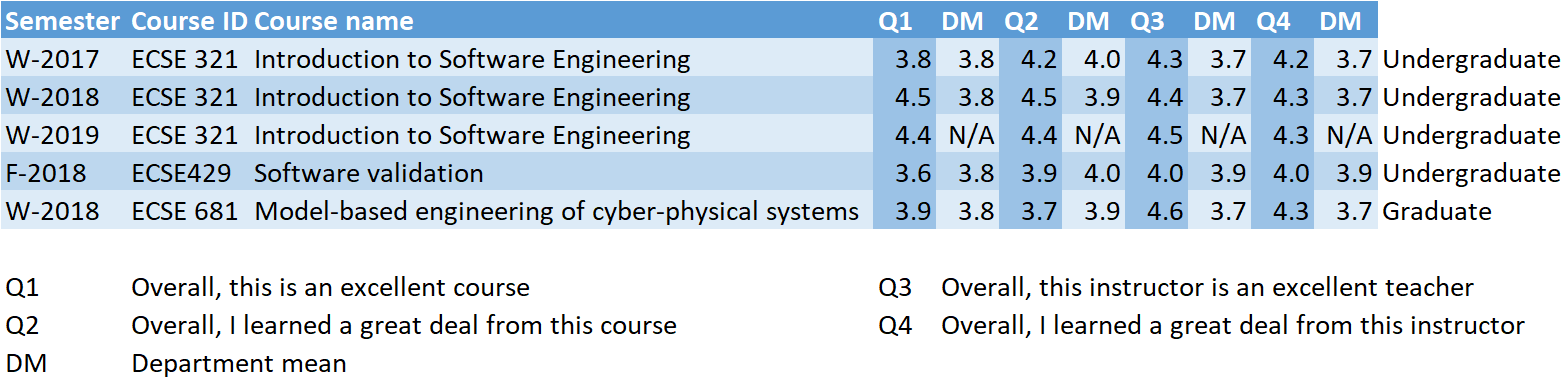
\includegraphics[width=\textwidth]{figures/TeachingEval}
\caption{Results of course evaluations at McGill University}
\label{fig:course-eval}
\end{table}


%\cvsubsection{Taught Courses at McGill University (Instructor and course co-developer)}

%Introduction to Software Engineer (undergraduate, 75-90 students, 2017 Winter, 2018 Winter)

%Model based engineering of cyber-physical systems (this is the new course name - graduate, 18 students, 2018 Winter)

%\begin{figure}
%\centering
%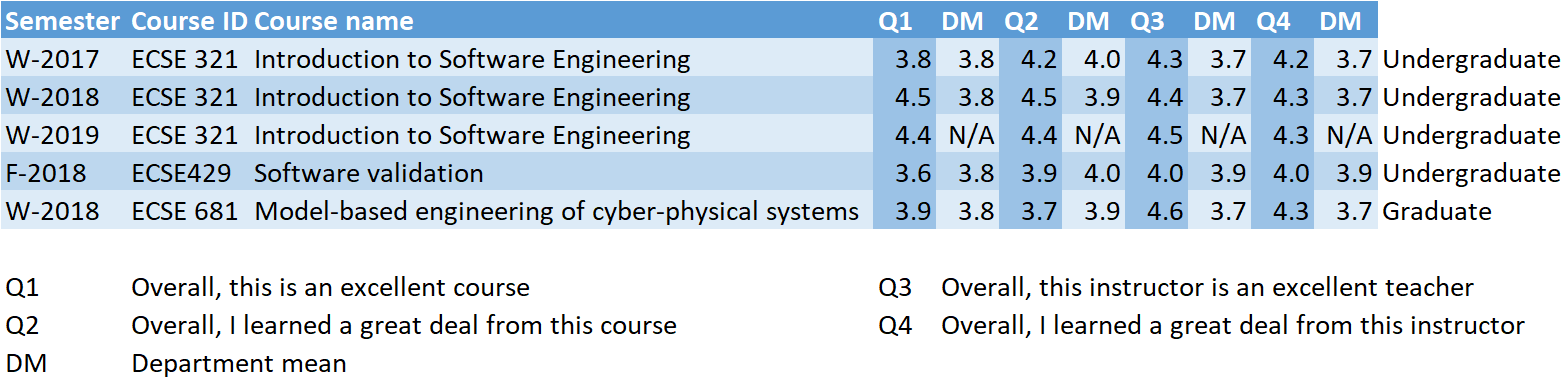
\includegraphics[width=.9\textwidth]{figures/TeachingEval}
%\caption{Results of teaching evaluation at McGill University}
%\end{figure}

%\cvsubsection{Taught Courses at BME (Lecturer and course co-developer)}
%
%Model driven system development (2010-, MSc, 15-25 students)
%
%Model driven software development (2010-2014, MSc, 10-20 students)
%
%UML-based modeling and analysis (2002 - 2008, MSc, 70-80 students / year)
%
%Open development frameworks (2005 - 2008, MSc, 10-20 students)
%
%Foundations of model-driven development (2005- , PhD, 5-10 students)
%
%(All these courses were taught for students of software engineering specialized in dependable systems)
%
%\cvsubsection{Supervised Courses}
%
%Systems engineering (2016- , BSc, 60-80 students)
%
%System integration (2010- , MSc, 10-20 students)
%
%Eclipse-based based development and integration (2010- , MSc, 10 students) 
%
%Eclipse technologies (2009- , BSc, 10-20 students) 
%
%\cvsubsection{Participating as Lecturer}
%
%Formal methods (2001 - 2006, BSc, 300-450 students)
%
%\cvsubsection{Teaching Assistant}
% 
%Formal languages (1999 - 2001, BSc, 20-30 students)
%
%Fault tolerant systems lab (200 - 2001, BSc, 30 students)


%\cvsection{Spoken Languages}
%Hungarian (mother tongue) \\ 
%English (fluent) \\ 
%French (intermediate, B2/C1)

\newpage

\cvsection{Services to the Scientific Community}
\lhead{Services to the Scientific Community} 
%\cvsubsection{Program Co-Chair}

\begin{refsection}
\newrefcontext[labelprefix=CH]
\nocite{mise2019-chair,sle2016-chair,icmt2014-chair,fase2013-chair,amt2012-chair,agtive2011-chair,grabats2010-chair,gtvmt2006-chair,grabats2006-chair}
\printbibliography[title=Program Co-Chair]
\end{refsection}

\begin{refsection}
\newrefcontext[labelprefix=SC]
\nocite{etaps2008-sc,etaps2013-sc,icmt2014-sc}
\printbibliography[title=Steering Committee Member]
\end{refsection}

\begin{refsection}
\newrefcontext[labelprefix=LO]
\nocite{icse2019post-chair,staf16ws-chair,staf2015ds-chair,staf2013-chair,models2012-chair,sensus2009-lo,etaps2008-lo,models2007-chair,edcc2005-lo}
\printbibliography[title=Chair of Organizing Committees]
\end{refsection}

\begin{refsection}
\newrefcontext[labelprefix=DS]
\nocite{Haussler,Oakes,AlBayati,Beyhl,GasconSamson,DeCarlos,Hegyhati,Vajk,Ciccozzi,Kalauz,Hildebrandt,Zombori,Guta,Siikarla,Lundkvist,Meszaros,Gergely,Vidacs,Hettel,Sipos,Lukacsy,Hajdara}
\printbibliography[title=Participation in PhD Defense Committees]
\end{refsection}

\cvsection{Program Committee Membership}

\begin{refsection}
\newrefcontext[labelprefix=SE]
  \nocite{models2019-pc,ecmfa-2019-pc,icse2019-pc,%
icse2018-pc,fase2018-pc,icmt2018-pc,ecmfa2018-pc,models2018-pc,securemde2018-pc,%
models2017-pc,fase2017-pc,icmt2017-pc,ase2017tools-pc,mise2017-pc,%
ase2016-pc,models2016-pc,ecmfa2016-pc,models2016ds-pc,icmt2016-pc,%
ase2015-pc,models2015-pc,sle2015-pc,fase2015-pc,%
ase2014-pc,models2014-pc,fase2014-pc,%
  models2013-pc,ecmfa2013-pc,%
  models2012-pc,ase2012-pc,ase2012tools-pc,icse2012tools-pc,%
  fase2012-pc,csmr2012-pc,ecmfa2012-pc,icmt2012-pc,%
  ase2011-pc,ase2011tools-pc%
  models2011-pc,fase2011-pc,icmt2011-pc,ecmfa2011-pc,sofsem2011-pc,%
  mbsdi2011-pc,melo2011-pc,%
  models2010-pc,fase2010-pc,icmt2010-pc,ase2010-pc,modelsedu2010-pc,%
  models2009-pc,fase2009-pc,icmt2009-pc,ase2009-pc,%
  models2008-pc,icmt2008-pc,aramis2008-pc,%
  wapl2007-pc,modelsedu2007-pc,modeva2007-pc,atem2007-pc,sac2007-pc,%
  sac2006-pc,iwmec2006-pc,modeva2006-pc,atem2006-pc,gramot2006-pc,cmt2006-pc,gamma2006-pc,%
  mtip2005-pc,gramot2005-pc%
  }
\printbibliography[title=Software Engineering]
\end{refsection}

\begin{refsection}
\newrefcontext[labelprefix=VT]
  \nocite{gam2015-pc,vlhcc2014-pc,vlhcc2013-pc,vlhcc2012-pc,gtvmt2012-pc,%
  vlhcc2011-pc,gtvmt2011-pc,%
  gtvmt2010-pc,%
  gtvmt2009-pc,%
  gtvmt2008-pc,grabats2008-pc,%
  gtvmt2007-pc,agtive2007-pc,%
  fujaba2006-pc,fujaba2005-pc,grabats2004-pc%
  }
\printbibliography[title=Visual Modeling Techniques and Tools]
\end{refsection}

\begin{refsection}
\newrefcontext[labelprefix=FM]
  \nocite{sefm2019-pc,facs2018-pc,fmmdd2016-pc,icgt2014,icgt2012-pc,icgt2012ds-pc,%
  ictac2011-pc,icgt2010-pc,ictac2010-pc,%
  fm2009-pc,%
  icgt2008-pc,pngt2008-pc,%
  icgt2006-pc,gtvc2006-pc,gtvc2005-pc}
\printbibliography[title=Formal Methods]
\end{refsection}


\begin{refsection}
\newrefcontext[labelprefix=DC]
  \nocite{ewdc2011-pc,dsn2009-pc,edcc2006-pc,icdcs2006-pc}
\printbibliography[title=Dependable Computing]
\end{refsection}

\begin{refsection}
\newrefcontext[labelprefix=ED]
\nocite{models2010edu-pc,models2007edu-pc}
\printbibliography[title=Education]
\end{refsection}

\begin{refsection}
\newrefcontext[labelprefix=JR]
\nocite{sosym,jot,scp,ieee-tse,jss,ieee-sw,acm-tosem,sttt,ause}
\printbibliography[title=Journals]
\end{refsection}

\begin{refsection}
\newrefcontext[labelprefix=IJ]
\nocite{cost,nwo,nserc,fct,fwf,mta,simi,york,stellenbosch,udem}
\printbibliography[title=International Juries and Evaluation]
\end{refsection}


%\newpage
\cvsection{Publication highlights}
%\lhead{Publication list} 

Total number of papers: 166 \\
%Books and book chapters: 9 \\
%Peer reviewed (regular and electronic) journal papers: 45 \\
%Peer reviewed journal papers (incl. peer reviewed electronic journals): 35  (46) \\
%(incl. 10 in Software and Systems Modeling, Springer) \\
%Peer reviewed conference (+ workshop) papers: 69 (+33)  \\
%Refereed workshop papers: 31: \\
Number of citations: 6572 (as of May 25th, 2019 by Google Scholar) \\
%Number of citations: 3613 (as of November 30th, 2014 by CIDS 3.0) \\
%(of which in Scopus: 839, in MTMT: 1501) \\ 
%h-index (by CIDS): 31, g-index (by CIDS): 56, h-index (in MTMT): 26,\\
h-index (by Google Scholar): 41 \\
Source: \url{http://scholar.google.pt/citations?user=4Ya6dVoAAAAJ}  \\
DBLP: \url{https://dblp.uni-trier.de/pers/hd/v/Varr=oacute=:D=aacute=niel}  \\
%\url{http://cids.fc.ul.pt/cids_3_0/results.php?acc=3741130101140333046} \\
%\url{https://vm.mtmt.hu/www/index.php?AuthorID=10001355}
%ResearchNet: \url{https://www.researchgate.net/profile/Daniel_Varro/publications}
%\url{http://cids.di.fc.ul.pt/cids_3_0/results.php?acc=19271126111105329059}

110 of my papers had a student co-author I supervised or co-supervised. \\
All papers which received a distinguished paper award had a student co-author \\
I had joint paper with 144 co-authors (DBLP data). \\

%\begin{table}[htb]
%\begin{tabular}{@{}lllll@{}}
%\toprule
%\textbf{Publications} & \textbf{Lifetime} (20y) & \textbf{McGill} (3y) & \textbf{Student co-author} \\ \midrule
%Journals & 45 & 6 & 28 \\ \midrule
%Book chapters & 9 & 1 & 6  \\ \midrule
%Conferences & 68 & 16 & 54  \\ \midrule
%Workshops & 33 & 2 & 20  \\ \midrule
%Other & 3 & 0 & 2  \\ \midrule
%Invited & 7 & 0 & N/A   \\ \midrule
%Edited & 10 & 1 & N/A \\ \midrule
%PhD theses &  9 & 1 & All \\ \midrule
%\bottomrule
%\end{tabular}
%\caption{Publication overview (Lifetime: 20 years, McGill: 3 years)}
%\label{tab:publication-overview}
%\end{table}

%\cvsection{References}
%
%\begin{enumerate}
%\item Prof. Dr. Gregor Engels (engels@upb.de) \\
%Full professor \\
%Datenbank- und Informationssysteme, Universität Paderborn \\
%Warburger Str. 100, 33098 Paderborn 
%
%\item Prof. Reiko Heckel (reiko@mcs.le.ac.uk) \\
%Professor of Computer Science, Head of Department \\
%G11 Informatics Building, \\
%Department of Informatics, University of Leicester, \\
%University Road, Leicester, LE1 7RH
%
%\item Prof. Arend Rensink (arend.rensink@utwente.nl) \\
%Full professor \\
%Department of Computer Science, University of Twente \\
%P.O. Box 217, NL-7500 AE Enschede
%
%\item Prof. Dr. rer. nat. Andy Schürr (Andy.Schuerr@es.tu-darmstadt.de) \\
%Full professor \\
%Institute for Data Technology, Dept. for Electrical Engineering and Communication Technology, \\
%Darmstadt University of Technology \\
%Magdalenenstr. 4, 64289 Darmstadt
%\end{enumerate}




%\cvsection{Detailed publication list}

%In software engineering (and particular, in my research area), publishing in top conferences is as important as publishing in top journals. 
%\emph{Comments to publication list:} Names of students who worked under my supervision (or co-supervision) at the time of publication are marked with \textsuperscript{*}. The first author of a paper is frequently a graduate student who made the most direct contribution to the research. The last author is typically the supervisor who signs the research program. However, other policies of authorship are also common in case of cross-institutional collaborations (e.g. alphabetical order, mixed alphabetical, etc.). 

%
%For most top conferences, the acceptance rate is published which is typically below 33\%.  


\begin{refsection}
\newrefcontext[labelprefix=B]
  \nocite{fmi2004,nagl65-2010,bpel2sal-sensoria-book,sensoria-uml,SENSORIABook:AdvancesInGT,mdegt2005_ggzvvv,caise2011-revised,fmic2005_pv,fmhe2018}
\printbibliography[title=Books and Book Chapter (Total: 9)]
\end{refsection}


\begin{refsection}
\newrefcontext[labelprefix=J]
  \nocite{SCP2002,GRABATS2002j,GTVMT2003j,sosym2003_vpm,pp2003_as,FundInf2003_ghv,%
sosym2004_mc,gtvmt2004-gsv-j,gtvmt2004-vv-j,grabats2004-vfv-j,%
sosym2005_db,gramot2005-j,gramot2005-tax-j,%
sosym2005_bhtv,pngt2006-vv,gramot2006-j,hiradas2006-hvv,%
scp-2007,GT-VMT2007-hvv,gtvc2006-gkv,gtvmt2006-dpv-j,%
ijcsse08-kgv,Gonczy-safecert08,sosym2008-mtbe,%
Rath-sosym09,Bergmann-gtvmt09,%
Bergmann-sttt10,Gilmore-sosym10,eceasst2010-guided,eceasst2011-type,%
sosym2012-tools,sosym2011-cdt,sosym2011-csp,scp2015,ause2015,ist2015,sosym2016-trace,sosym2017-dsl,sosym2018-cep,sosym2016-viatra-invited,sosym2017-mondo,sosym2017-tb,act2017,sosym2018-mt,ieeesw2018} 
\printbibliography[title=Refereed Journals incl. Electronic Journals (Total: 45)]
\end{refsection}
 
\begin{refsection}
\newrefcontext[labelprefix=C]
  \nocite{UML2002,ASE2002,ICGT2002-GHV02,ICGT2002-SC,%
esec03_bhtv,uml2003_tool,%
wicse2004_bhtv,GI2004,icgt2004_rsv,uml2004_meta,%
isas05_bvp,fase2005_eeltvv,vlhcc05_vsv,%
sac06_vtcl,sac06_plugin,isas2006_kvn,models2006-varro,icgt2006,%
agtive07-vhv,isas-2007-kv,sac2007-vb,%
icgt08-bhrv,Gonczy-mdwe08,icmt08-rbov08,Rath-vlhcc08,%
Bergmann-icmt09,Horvath-models09,Rath-models09,%
SEFM10:back-ann,models-2010-incquery,%
ase2011-dse,ase2011-mtslice,ase2011-tool,vlhcc2011,ecmfa2011,icmt2011,ServiceWave2011,%
models2012,ecmfa2012,icgt2012-ts,icst2012,tools2012,models2013,%
ase2014,models2014-iqd,models2014-stream,sle2014,csmr2014,%
icmt2015,icgt2015,%
fase2016-solver,fase2016-merge,icgt2016,MODELS2016-access,MODELS2016-bx,MODELS2016-metrics,%
esec-fse2017,models2017,adbis2017,icmt2017,%
icse2018-solver,icse2018-gamma,fase2018-diverse,fase2018-cps,models2018,vlhcc2018,nfm2018,models2018-tool,%
icse2019-tool} 
\printbibliography[title=Peer Reviewed Conference Papers (Total: 69)]
\end{refsection}

\begin{refsection}
\newrefcontext[labelprefix=O]
  \nocite{dasc2010-hvs,Daboczi-AWSN2013,dasc2014}
\printbibliography[title=Other Conference Papers (Total: 3)]
\end{refsection}


\begin{refsection}
\newrefcontext[labelprefix=W]
  \nocite{GRATRA2000,DDECS2000,WTUML01,%
edcc2002_svp,FMOODS2002,AGT2002,%GRABATS2002,GTVMT2002,
cbse03_bhtv,DDECS2003_tvp,csduml2003,%
%grabats2004_vfv,gtvmt04_vv,gtvmt04_gsv,
mtip2005,%gramot2005_tax,gramot2005_adapt,gramot2006-vvs,
cmt2006,wsmate2006,dspd2006_rv,models2006-edu,%pngt2006-vv,gtvc2006-gkv,gtvmt06_dpv,
efts-2007-kgv,%GT-VMT2007-hvv,
gramot08-borvv,%Gonczy-safecert08,
%Bergmann-gtvmt09,
SEFM10ToolDemo:back-ann,%eceasst2010-guided,
ocl2012,amt2012-query,%
Kolovos-bigmde2013,Izso-bigmde2013,%
bigmde2014,cmseba2014,mpm2014,oss4mde2014,vao2014,%
staf2015-project,ttc2015,gemoc2015,%
BX2016,STAF-proj-2016,commitmde2016,%
commitmde2017}
\printbibliography[title=Refereed Workshop Papers (Total: 33)]
\end{refsection}
  

\begin{refsection}
\newrefcontext[labelprefix=I]
  \nocite{easst2006-etv,Wirsing-isola08,agtive07-toolcontest,models09-edu,csmr2012-invited,sofsem2016-invited,pame2015}
\printbibliography[title=Invited Papers (Total: 7)]
\end{refsection}

\begin{refsection}
\newrefcontext[labelprefix=E]
  \nocite{gtvmt2006,icgt2006-grabats,grabats2010,agtive2011,amt2012,fase2013,icmt2014,staf2015-ds,sle2016,staf2016-ws}
\printbibliography[title=Edited Volumes (Total: 10)]
\end{refsection}


%For most top conferences, the acceptance rate is published which is typically below 33\%.  

%\begin{refsection}
%\newrefcontext[labelprefix=B]
%  \nocite{fmi2004,nagl65-2010,bpel2sal-sensoria-book,sensoria-uml,SENSORIABook:AdvancesInGT,mdegt2005_ggzvvv,caise2011-revised,fmic2005_pv,fmhe2018}
%\printbibliography[title=Books and Book Chapter (Total: 9)]
%\end{refsection}
%
%
%\begin{refsection}
%\newrefcontext[labelprefix=J]
%  \nocite{SCP2002,GRABATS2002j,GTVMT2003j,sosym2003_vpm,pp2003_as,FundInf2003_ghv,%
%sosym2004_mc,gtvmt2004-gsv-j,gtvmt2004-vv-j,grabats2004-vfv-j,%
%sosym2005_db,gramot2005-j,gramot2005-tax-j,%
%sosym2005_bhtv,pngt2006-vv,gramot2006-j,hiradas2006-hvv,%
%scp-2007,GT-VMT2007-hvv,gtvc2006-gkv,gtvmt2006-dpv-j,%
%ijcsse08-kgv,Gonczy-safecert08,sosym2008-mtbe,%
%Rath-sosym09,Bergmann-gtvmt09,%
%Bergmann-sttt10,Gilmore-sosym10,eceasst2010-guided,eceasst2011-type,%
%sosym2012-tools,sosym2011-cdt,sosym2011-csp,scp2015,ause2015,ist2015,sosym2016-trace,sosym2017-dsl,sosym2018-cep,sosym2016-viatra-invited,sosym2017-mondo,sosym2017-tb,act2017,sosym2018-mt,ieeesw2018} 
%\printbibliography[title=Refereed Journals incl. Electronic Journals (Total: 45)]
%\end{refsection}
% 
%\begin{refsection}
%\newrefcontext[labelprefix=C]
%  \nocite{UML2002,ASE2002,ICGT2002-GHV02,ICGT2002-SC,%
%esec03_bhtv,uml2003_tool,%
%wicse2004_bhtv,GI2004,icgt2004_rsv,uml2004_meta,%
%isas05_bvp,fase2005_eeltvv,vlhcc05_vsv,%
%sac06_vtcl,sac06_plugin,isas2006_kvn,models2006-varro,icgt2006,%
%agtive07-vhv,isas-2007-kv,sac2007-vb,%
%icgt08-bhrv,Gonczy-mdwe08,icmt08-rbov08,Rath-vlhcc08,%
%Bergmann-icmt09,Horvath-models09,Rath-models09,%
%SEFM10:back-ann,models-2010-incquery,%
%ase2011-dse,ase2011-mtslice,ase2011-tool,vlhcc2011,ecmfa2011,icmt2011,ServiceWave2011,%
%models2012,ecmfa2012,icgt2012-ts,icst2012,tools2012,models2013,%
%ase2014,models2014-iqd,models2014-stream,sle2014,csmr2014,%
%icmt2015,icgt2015,%
%fase2016-solver,fase2016-merge,icgt2016,MODELS2016-access,MODELS2016-bx,MODELS2016-metrics,%
%esec-fse2017,models2017,adbis2017,icmt2017,%
%icse2018-solver,icse2018-gamma,fase2018-diverse,fase2018-cps,models2018,vlhcc2018,nfm2018,models2018-tool,%
%icse2019-tool} 
%\printbibliography[title=Peer Reviewed Conference Papers (Total: 69)]
%\end{refsection}
%
%\begin{refsection}
%\newrefcontext[labelprefix=O]
%  \nocite{dasc2010-hvs,Daboczi-AWSN2013,dasc2014}
%\printbibliography[title=Other Conference Papers (Total: 3)]
%\end{refsection}
%
%
%\begin{refsection}
%\newrefcontext[labelprefix=W]
%  \nocite{GRATRA2000,DDECS2000,WTUML01,%
%edcc2002_svp,FMOODS2002,AGT2002,%GRABATS2002,GTVMT2002,
%cbse03_bhtv,DDECS2003_tvp,csduml2003,%
%%grabats2004_vfv,gtvmt04_vv,gtvmt04_gsv,
%mtip2005,%gramot2005_tax,gramot2005_adapt,gramot2006-vvs,
%cmt2006,wsmate2006,dspd2006_rv,models2006-edu,%pngt2006-vv,gtvc2006-gkv,gtvmt06_dpv,
%efts-2007-kgv,%GT-VMT2007-hvv,
%gramot08-borvv,%Gonczy-safecert08,
%%Bergmann-gtvmt09,
%SEFM10ToolDemo:back-ann,%eceasst2010-guided,
%ocl2012,amt2012-query,%
%Kolovos-bigmde2013,Izso-bigmde2013,%
%bigmde2014,cmseba2014,mpm2014,oss4mde2014,vao2014,%
%staf2015-project,ttc2015,gemoc2015,%
%BX2016,STAF-proj-2016,commitmde2016,%
%commitmde2017}
%\printbibliography[title=Refereed Workshop Papers (Total: 33)]
%\end{refsection}
%  
%
%\begin{refsection}
%\newrefcontext[labelprefix=I]
%  \nocite{easst2006-etv,Wirsing-isola08,agtive07-toolcontest,models09-edu,csmr2012-invited,sofsem2016-invited,pame2015}
%\printbibliography[title=Invited Papers (Total: 7)]
%\end{refsection}
%
%\begin{refsection}
%\newrefcontext[labelprefix=E]
%  \nocite{gtvmt2006,icgt2006-grabats,grabats2010,agtive2011,amt2012,fase2013,icmt2014,staf2015-ds,sle2016,staf2016-ws}
%\printbibliography[title=Edited Volumes (Total: 10)]
%\end{refsection}



% Automatically Generated Bibliography

%\cvsection{Family and Hobbies}
%married and proud father of two sons (6 and 4 years old) \\
%
%futsal (indoor soccer); \years{1997-2003, 2010-} goalkeeper in 1st and 2nd
%league of the Hungarian National Futsal Championship \\
%
%music (singing in choirs, and participating in concerts for children)

%\nocite{*}\bibliographystyle{ieeetr}
%\bibliography{bib/pcmember,bib/varrodan}

\end{document}